\section{The \appName Scheme} \label{sec:m}

\subsection{Encoding}

\paragraph{Overview.}

Segmentation datasets contain two important pieces of information across the image stack: per-segment shape and per-pixel label. 
Decoupling these two components allows for better compression on each.

\paragraph{Boundary Encoding.}
\label{sec:boundary-map}

To encode the segment shapes, we consider the boundary pixels between two segments. 
Removing the per-pixel labels, we produce a boundary map for each slice where a pixel $(x, y, z)$ is 1 if either pixel at $(x + 1, y, z)$ or $(x, y + 1, z)$ belongs to a different segment. 
The boundary map is divided into non-overlapping congruent 3D windows. If there are $n$ pixels per window, each window $w$ is assigned an integer $V_w \in [0, 2^n)$ where $V_w$ is defined as:

\begin{equation}
V_w = \sum_{i = 0}^{n - 1} \mathbb{I}(i) 2^i,
\end{equation}

\noindent
and $\mathbb{I}(i)$ is 1 if pixel $i$ is on a boundary and 0 otherwise. 
Figure~\ref{fig:bockwurst-encoding} shows an example segmentation with a window size of $4 \times 4 \times 1$.

\begin{figure}[h]
  \begin{center}
    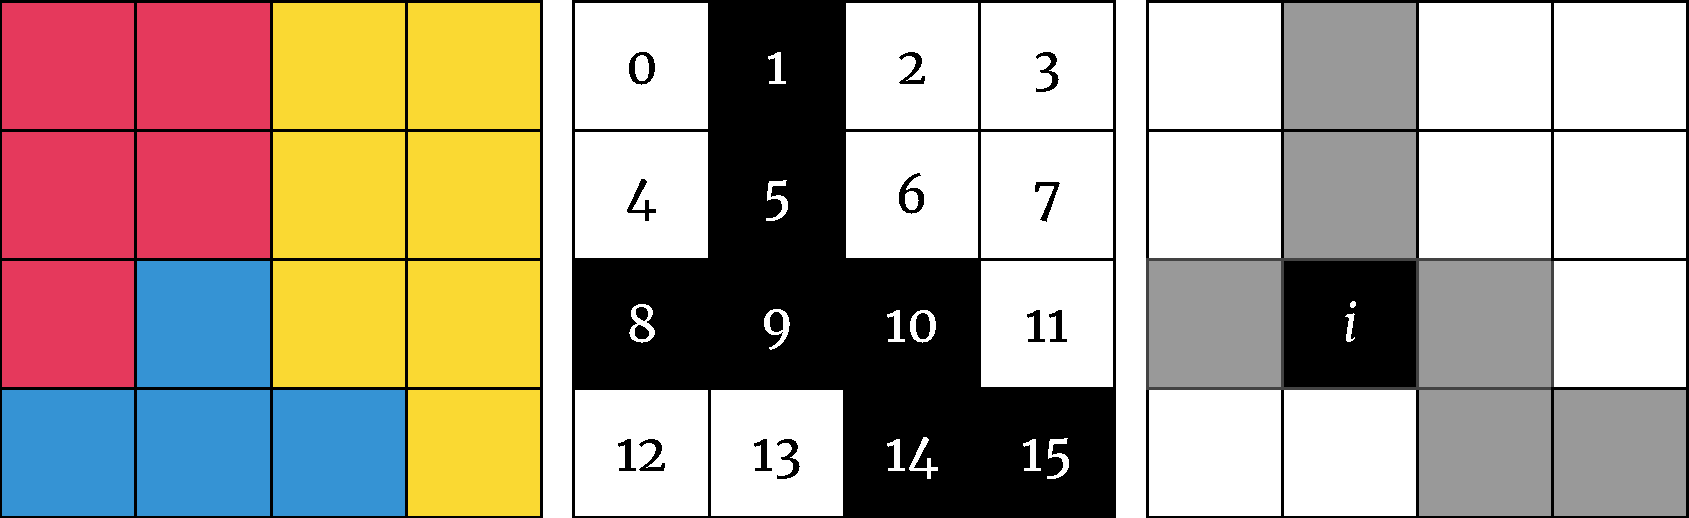
\includegraphics[width=0.7\textwidth]{gfx/encoding_diagram_opt.pdf}
  \end{center}
  \caption{A $4 \times 4 \times 1$ pixel window where three unique labels meet (left). The boundary map for the same window, where dark pixels represent the boundary (center). This window has an encoded value of 50,978 $(2^1 + 2^5 + 2^8 + 2^9 + 2^{10} + 2^{14} + 2^{15})$. A boundary pixel $i$ that is indeterminate and requires additional decoding information (right).}
  \label{fig:bockwurst-encoding}
\end{figure}

A priori, each window could take any of $2^n$ distinct values, and therefore require $n$ bits to encode without further manipulation. 
However, boundaries in segmentation images are not random, and many of these values never appear. 
Indeed, we find that a small subset of high-frequency $V_w$ values accounts for most windows, allowing for significant compression. 
Figure~\ref{fig:bockwurst-frequency} shows the 100 most common windows for a representative connectomics dataset. 
These 100 frequently occurring windows account for approximately 82\% of the over 1.2 million $V_w$ values in this dataset.
Nearly all of these windows correspond to simple lines traversing through the window. 
For contrast, we also provide 5 randomly generated windows that never occur in the dataset.

We define $N$ as the number of distinct $V_w$ representing all of the windows in an image stack. 
We construct an invertible function $f(V_w) \to [0, N)$ to transform the window values into a smaller set of integers. 
For all real-world segmentations $N \ll 2^n$; however, we assume no constraint on $N$ in order to guarantee lossless compression. 
With this function, each $V_w$ requires $\log_2{N}$ bits of information to encode. 
This is fewer than the initial number of bits so long as $N \leq 2^{n - 1}$.  
We create two arrays that store the per-segment shape encoding: $\texttt{WindowValues[]}$ contains the value $f(V_w)$ for every window $w$ and $\texttt{ValueMapping[]}$ contains the reverse mapping from $[0, N) \to [0, 2^n)$ based on the function $f$. 
Long sequences of $0$s in $\texttt{WindowValues[]}$ are reduced using run-length encoding.
%\vspace{-1mm}
\paragraph{Per-Pixel Label Compression.}

So far we have focused exclusively on transforming the boundary map of an image segmentation. 
However, the per-pixel labels themselves are equally important. 
The boundary map divides each image slice into different segments. 
By design, all pixels in the same segment have the same label so we store only one label per segment for each slice. 
We use a connected-component labeling algorithm to store one label per segment \cite{he2009fast}. 
The algorithm labels all pixels clustered within a component $m$ from $M$ section labels.
We store the original label for a segment $m$ in slice $z$ in $\texttt{Labels}_z\texttt{[m]}$. 
We concatenate these arrays for every image slice to create a variable $\texttt{Labels[]}$.
%\vspace{-1mm}
\paragraph{Exceptions.}

\begin{figure}
  \begin{center}
    \begin{minipage}{.8\linewidth}
      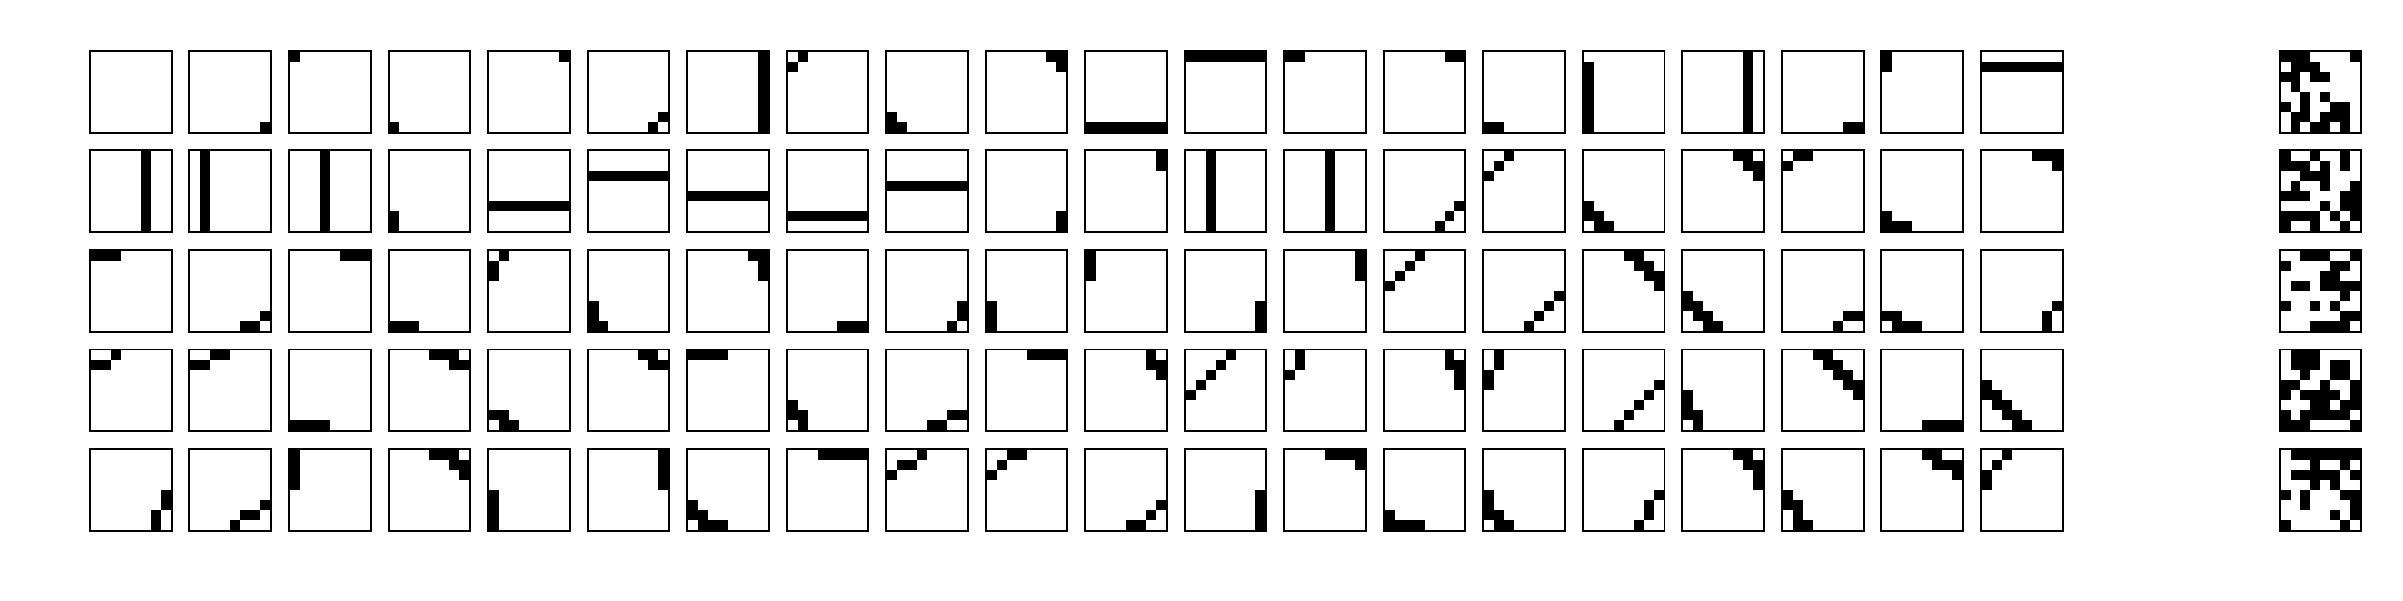
\includegraphics[width=\linewidth]{./gfx/window_values.pdf}
    \end{minipage}
  \end{center}
  \caption{The 100 most frequent windows accounting for approximately 82\% of the over 1.2 million $V_w$ values on a representative connectomics dataset contrasted with 5 randomly generated windows. Each box represents an 8 x 8 x 1 window where black pixels are boundary and white pixels are non-boundary.}
  \label{fig:bockwurst-frequency}
\end{figure}

Thus far, we have assumed the boundaries described in Section~\ref{sec:boundary-map} provide enough information to reconstruct the entire segmentation.
Pixels not on a segment boundary are easily relabeled using the $\texttt{Labels[]}$ array. 
However, more care is needed for pixels on the segment boundaries. 
Consider Figure~\ref{fig:bockwurst-encoding}, which depicts a difficult boundary to decode. 
If a boundary pixel has a non-boundary neighbor to the left or above, then that pixel merely takes on the value of that neighbor. 
However, the pixel $i$ requires more care since its relevant neighbors are both boundary pixels. 
If a non-boundary neighbor pixel shares a label with the undetermined pixel, we add the offset to that neighbor to an array \texttt{IndeterminateValues[]}. 
Otherwise we add that per-pixel label.
%\vspace{-1mm}
\paragraph{Metadata.}

We construct a data structure containing the two per-segment shape and two per-pixel label arrays. The last component of the data structure is the \texttt{Header}, which contains the dimensions of the original data, the window size, and the size of the arrays. \appName could be improved by further compressing the individual components of the encoding (e.g., Huffman encoding the $V_w$ values). We achieve strong overall compression by using a second-stage general compression scheme such as LZMA~(Sec.~\ref{sec:results}).


\subsection{Decoding}

The first step in decoding the data is to reconstruct the boundary map. We iterate over every pixel, determine the corresponding window $w$, and retrieve the encoded window value $f(V_w)$ from the $\texttt{WindowValues[]}$ array. These values range from $0$ to $N - 1$ and correspond to an index in $\texttt{ValueMapping[]}$ that contains the original $V_w$ value. After decoding $V_w$, the value of pixel $i$ in window $w$ equals $V_w \land 2^i$.

After reproducing the boundary map, we execute the same deterministic connected-components algorithm per slice as when encoding. Each component in the boundary map receives a label between $0$ and $M - 1$. Using the $\texttt{Labels[]}$ array, we can easily translate these component labels into the original per-pixel labels for every slice. To determine the per-pixel labels for every boundary pixel, we iterate over the entire dataset in raster order. Any boundary pixel $(x, y, z)$ with a non-boundary neighbor at $(x - 1, y, z)$ or $(x, y - 1, z)$ shares the same per-pixel label. If both relevant neighbors are boundaries we consider the next unused value in the $\texttt{IndeterminateValues[]}$ array and update this pixel's label.

\subsection{Complexity}

In what follows, $P$ is the number of input pixels; $N$ is the number of distinct window values; $X$, $Y$ and $Z$ are the size of the $x$, $y$, and $z$ dimensions of the input data;  and $\alpha$ is the inverse Ackermann function~\cite{fredman1989cell}.
%\vspace{-5mm}
\paragraph{Encoding.}

Extracting the boundaries from the segmentation, generating the $V_w$ values, and populating the $\texttt{IndeterminateValues[]}$ array are all linear work in $P$. The $N$ unique window values are sorted to create the $\texttt{ValueMapping}$ variable. Generating the $\texttt{Labels[]}$ array requires running a connected-component labeling algorithm over each $z$ slice; we use a union-find data structure with union by rank and path compression optimizations.  The overall complexity of the compression scheme is therefore $O\left({P(1 + \alpha(XY)) + N\log{N}}\right)$.
%\vspace{-5mm}
\paragraph{Decoding.}

Decoding the window values, reconstructing the boundary map, and applying the correct per-pixel labels for all boundary pixels using the array \texttt{IndeterminateValues[]} are all linear work in $P$.  Reconstructing the per-pixel labels requires running the connected-component labeling algorithm over every image slice. The overall complexity of the decompression scheme is therefore $O\left({P(1 + \alpha(XY))}\right)$.

%\subsection{Complexity}
%
%\paragraph{Encoding.}
%
%Extracting the boundaries from the segmentation and generating the $V_w$ values is linear in the number of input pixels $P$. The $N$ unique window values are sorted to create the $\texttt{ValueMapping}$ variable. Generating the $\texttt{IDs}$ array requires running a connected-component labeling algorithm over each $z$ slice. The algorithm uses a union-find data structure with union by rank and path compression optimizations. Populating the $\texttt{IndeterminateValues}$ array is linear in the number of pixels. With $X$, $Y$ and $Z$ as the size of the $x$, $y$, and $z$ dimensions of the input data, $N$ as the number of unique window values, and $P$ as the number of pixels, the complexity of the compression scheme is $O\left({P(1 + \alpha(XY)) + N\log{N}}\right)$, where $\alpha$ is the inverse Ackermann function\cite{Fredman:1989:CPC:73007.73040}.
%
%\paragraph{Decoding.}
%
%Decoding the window values and reconstructing the boundary map is linear in the number of input pixels $P$. Reconstructing the per-pixel labels requires running the connected-component labeling algorithm over every image slice. Applying the correct per-pixel labels for all boundary pixels using $\texttt{IndeterminateValues}$ is linear in the number of input pixels. With $X$ and $Y$ as the size of the $x$ and $y$ dimensions, and $P$ as the number of pixels, the complexity of the decompression scheme is $O\left({P(1 + \alpha(XY))}\right)$.
